%% Cancers (MDPI) — Research Article
%% Compile: xelatex (twice)
\documentclass[12pt,a4paper]{article}

\usepackage{graphicx}
\usepackage{booktabs}
\usepackage{amsmath}
\usepackage{geometry}
\usepackage{hyperref}
\usepackage{microtype}
\usepackage{caption}
\usepackage{subcaption}
\usepackage{float}
\usepackage{setspace}
\usepackage{enumitem}
\usepackage{array}
\usepackage{xcolor}
\usepackage{titlesec}
\usepackage{authblk}
\usepackage{abstract}

\geometry{left=3cm, right=3cm, top=3cm, bottom=3cm}
\doublespacing

\hypersetup{
  colorlinks=true,
  linkcolor=blue!60!black,
  citecolor=blue!60!black,
  urlcolor=blue!60!black,
  pdftitle={Surgical Margin Status and Deep Learning-Identified Patient
    Subtypes as Prognostic Determinants in Esophageal Cancer:
    A Registry-Based Analysis with MICE Imputation}
}

\graphicspath{{../results/}}

\captionsetup{font=small, labelfont=bf, skip=6pt}

%% Section heading style
\titleformat{\section}{\normalfont\large\bfseries}{\thesection.}{0.5em}{}
\titleformat{\subsection}{\normalfont\normalsize\bfseries}{\thesubsection.}{0.5em}{}

\begin{document}

%%======================================================================
%% Title block
%%======================================================================
\begin{titlepage}
\vspace*{1cm}

\begin{center}
{\LARGE\bfseries Surgical Margin Status and Deep Learning--Identified
Patient Subtypes as Prognostic Determinants in Esophageal Cancer:
A Registry-Based Analysis with Multiple Imputation\par}

\vspace{1.2cm}

{\large
[Author 1 Name]\textsuperscript{1},
[Author 2 Name]\textsuperscript{1,2},
[Author 3 Name]\textsuperscript{1,*}\par}

\vspace{0.6cm}

{\normalsize
\textsuperscript{1}[Department of Surgery / Oncology],
[Institution Name], [City], Taiwan\\
\textsuperscript{2}[Second Affiliation, if applicable]\\[0.3em]
\textsuperscript{*}Correspondence: [email@institution.edu.tw];
Tel.: +886-X-XXXX-XXXX\par}

\vspace{1cm}

\textbf{Received:} [Date]; \textbf{Accepted:} [Date];
\textbf{Published:} [Date]

\vspace{0.3cm}
\textbf{Publisher's Note:} [Standard MDPI disclaimer]
\end{center}

\vspace{1.5cm}

%%----------------------------------------------------------------------
%% Abstract
%%----------------------------------------------------------------------
\noindent\rule{\linewidth}{0.4pt}
\vspace{0.3em}

\noindent\textbf{Abstract:}
\textbf{Background:} Esophageal cancer prognosis is poor; independent
prognostic determinants of surgical quality in Asian registry populations
remain incompletely characterised.
\textbf{Methods:} We analysed 2,367 esophageal cancer (ICD-10 C15)
cases from the China Medical University Hospital (CMUH) Cancer Registry (2006--2020) using Kaplan-Meier
analysis, multivariable Cox regression with MICE-imputed AJCC stage
(C-index 0.670), and unsupervised deep learning subtyping.
\textbf{Results:} The cohort was predominantly male (94.5\,\%; SCC,
85.4\,\%; median OS 13.4 months; 1,832 deaths). R0 resection margin
was the single robust modifiable predictor (HR 0.63, 95\,\%\,CI
0.55--0.73, $p < 0.001$). CCRT was non-significant under MICE
(HR 0.97, $p = 0.569$; unadjusted log-rank $p = 0.58$) but
significant in complete-case analysis of staged patients
(HR 0.72, $p < 0.001$); the $>$25\,\% divergence precludes a
definitive conclusion. Radical esophagectomy independently reduced
hazard (HR 0.61, $p < 0.001$). Deep learning identified three subtypes
--- mainstream SCC, adenocarcinoma-enriched, and
cervical/upper-oesophagus --- with no incremental OS value beyond
conventional classifiers ($\Delta$C-index $= -0.001$).
\textbf{Conclusions:} R0 resection margin attainment is the primary
modifiable prognostic determinant. CCRT benefit is method-sensitive;
prospective data with complete staging are required.

\vspace{0.5em}
\noindent\textbf{Keywords:} esophageal cancer; squamous cell carcinoma;
surgical resection; R0 margin; concurrent chemoradiotherapy; deep learning;
patient subtypes; CMUH Cancer Registry; hospital-based registry

\noindent\rule{\linewidth}{0.4pt}

\end{titlepage}

%%======================================================================
\section{Introduction}
%%======================================================================

Esophageal cancer is the seventh most common malignancy and the sixth
leading cause of cancer-related mortality worldwide, accounting for an
estimated 604,100 new cases and 544,076 deaths in 2020 \cite{Sung2021}.
Its global distribution is heterogeneous: squamous-cell carcinoma (SCC)
predominates in the ``esophageal cancer belt'' spanning northern Iran
through Central Asia to north-central China and in sub-Saharan Africa,
whereas esophageal adenocarcinoma has risen sharply in Western Europe
and North America, largely attributed to the epidemic of obesity and
gastroesophageal reflux disease \cite{Arnold2015, Lagergren2017}. In
Taiwan, esophageal cancer ranks among the top ten malignancies by
incidence, with a distinctive epidemiological profile driven by the
convergence of betel quid chewing, cigarette smoking, and alcohol
consumption --- the so-called ``three lifestyle risk triad'' --- that
confer synergistic carcinogenic effects on the esophageal squamous
epithelium \cite{Lee2005, Huang2018}.

The histological landscape of esophageal cancer in Asia differs
fundamentally from that in the West. SCC constitutes over 90\,\% of
esophageal malignancies in East and South-East Asia, while adenocarcinoma
accounts for fewer than 5\,\% \cite{Arnold2015}. This distinction carries
profound therapeutic implications: SCC typically arises in the middle and
upper esophagus, is more sensitive to chemoradiotherapy, and shares
carcinogenic pathways with head and neck cancers, whereas adenocarcinoma
clusters at the gastroesophageal junction and responds differently to
treatment paradigms \cite{Rustgi2014}. Understanding the clinical spectrum
of esophageal SCC in hospital-based registries is therefore essential for
optimising treatment protocols tailored to Asian patients.

Current management of resectable esophageal cancer is centred on
multimodal therapy. The landmark CROSS trial demonstrated that neoadjuvant
concurrent chemoradiotherapy (CCRT) followed by surgery significantly
improved overall survival (OS) compared with surgery alone (median OS 48.6
vs 24.0 months; HR 0.68, $p = 0.003$) \cite{vanHagen2012}. The FLOT4
trial established perioperative FLOT chemotherapy as standard of care for
gastroesophageal junction tumours in the West \cite{AlBatran2019}. For
unresectable or metastatic disease, immune checkpoint inhibitors ---
nivolumab (ATTRACTION-3, CheckMate~648), pembrolizumab (KEYNOTE-590) ---
have transformed the therapeutic landscape in SCC \cite{Kato2019,
Sun2021}. Despite these advances, the five-year survival rate remains
approximately 15--25\,\%, underscoring the need for better prognostic
stratification and personalised treatment allocation \cite{Kelly2021}. In
Taiwan, real-world data on surgical quality metrics --- resection margin
status, lymph node dissection extent, and their interaction with systemic
therapy --- remain incompletely characterised at population scale.

Machine learning and deep learning approaches have emerged as powerful
tools for discovering latent patient subgroups and prognostic features from
high-dimensional clinical data \cite{Kourou2015}. Autoencoders compress
complex clinical feature spaces into compact latent representations,
enabling unsupervised patient stratification via dimensionality reduction
techniques such as UMAP \cite{McInnes2018}. DeepSurv, a deep Cox
proportional-hazards network, extends conventional survival analysis to
non-linear feature interactions and provides interpretable feature
importance through permutation analysis \cite{Katzman2018}. To date, the
application of such methods to population-level cancer registry data in
Taiwan has been limited.

In this study we aimed to: (1) describe the clinical characteristics and
temporal trends of esophageal cancer in a large CMUH Cancer Registry
cohort spanning 2006--2020; (2) quantify the independent prognostic impact
of surgical modality, resection margin status, lymph node dissection extent,
and perioperative treatment sequencing on OS; (3) explore the relationship
between chemotherapy intensity and outcomes in the subset of patients with
available cycle data (noting that cumulative cycle documentation was
available in only 5.3\,\% of cases, precluding robust dose-response
inference); and (4) apply unsupervised deep learning to discover novel
patient subtypes with distinct biological and clinical profiles.

%%======================================================================
\section{Materials and Methods}
%%======================================================================

\subsection{Data source and cohort}
De-identified records were obtained from the long-form Taiwan Cancer
Registry dataset (2006--2020), which captures all newly diagnosed cancers
at hospitals in Taiwan \cite{MOHW2022}. The registry has been described
previously \cite{MHW2022registry}. We extracted all cases with ICD-10
topography code C15 (malignant neoplasm of the oesophagus) diagnosed
between 1 January 2006 and 31 December 2020. Cases with unknown sex or
negative follow-up duration were excluded. The final cohort comprised
2,367 patients.

\subsection{Clinical variables}
Tumour subsite was classified according to the ICD-O three-character
C-code (C15.0--C15.9). Histological subtype was derived from the
ICD-O morphology code: SCC (8070--8076), adenocarcinoma (8140, 8480,
8144), adenosquamous (8560), and carcinoma not otherwise specified (NOS;
8000, 8010, 8020). Differentiation grade was coded 1 (well) to 4
(undifferentiated). Clinical and pathological stage were coded using the
AJCC staging system; pathological stage superseded clinical stage when
available. Surgical modality was classified as: no surgery; endoscopic
resection (EMR/ESD); partial esophagectomy; or radical esophagectomy
(Ivor-Lewis or transhiatal; ICD-O procedure codes 51--55). Resection
margin was coded R0 (complete), R1 (microscopic positive), or R2
(macroscopic positive) from registry field 124. Lymph node extent was
classified across five ordinal levels (none through radical three-field).
Chemotherapy was classified by the registry's regimen field as: no
chemotherapy; single-agent; multi-agent; CCRT; or multi-agent plus
targeted/immunotherapy. Cumulative chemotherapy cycles were extracted
where recorded. Lifestyle variables (smoking, betel nut use, BMI) were
available for the subset with completed intake questionnaires.

\subsection{Overall survival and survival analysis}
Overall survival (OS) was defined as the time from date of diagnosis to
death from any cause, or last registry contact if alive. The event
indicator was coded 0 = dead (Taiwan registry convention) and 1 = alive.
Kaplan-Meier (KM) survival curves were generated for each categorical
predictor; groups were compared by the log-rank test (two-group) or
multivariate log-rank test (three or more groups). Statistical significance
was defined as $p < 0.05$.

\subsection{Multivariable Cox proportional hazards regression}
\label{sec:cox}
A multivariable Cox proportional hazards model was fitted with ridge
penalisation (penaliser $= 0.1$) to patients with complete data for all
covariates except AJCC stage. AJCC stage was encoded as three binary
indicator variables (Stage II, III, IV vs Stage I reference); patients
with unknown stage ($n = 609$) were coded zero on all stage indicators,
effectively grouping them with the Stage I reference stratum. This
approach retains stage-unknown patients in the model while avoiding
listwise deletion of a quarter of the cohort; it is reported as a
limitation (Section~\ref{sec:limitations}). AJCC stage was imputed using Multiple Imputation by Chained Equations
(MICE; Python \texttt{sklearn} \texttt{IterativeImputer}, estimator:
Extra Trees Regressor, 10 iterations, seed 42) with age, sex, histology,
subsite, surgical modality, margin status, CCRT, and chemotherapy as
predictors; imputed stage was rounded to the nearest integer and clamped
to the ordinal range I--IV. This replaces the zero-coding approach used
in earlier versions and constitutes the primary analysis. For comparison,
a sensitivity analysis using zero-coded stage (stage-unknown grouped with
Stage I reference, $n = 2{,}364$) is also reported.

The concordance (C-) index was computed from the fitted MICE model; a
bootstrap out-of-bag 95\,\% confidence interval was derived from $B =
500$ resamples applied to the MICE-imputed dataset (imputed stage values
held fixed; patient resampling only). Hazard ratios (HRs) with 95\,\%
confidence intervals (CI) are reported. Reference categories were:
Stage I, no surgery, R1/R2 margin, no CCRT, and single-agent or no
chemotherapy.

The proportional hazards (PH) assumption was evaluated for all covariates
using scaled Schoenfeld residuals (\texttt{lifelines.statistics.proportional\_hazard\_test},
rank transformation). For covariates where PH was violated ($p < 0.05$), a
time-split Cox model with a 12-month landmark was fitted as a supplementary
analysis: an \textit{early period} (0--12 months) and a \textit{late period}
($> 12$ months, restricted to survivors past the landmark). Results are
reported in Supplementary Table~S1.

\subsection{Unsupervised deep learning patient subtyping}
A symmetric autoencoder was trained on a standardised, median-imputed
feature matrix comprising age, sex, esophageal subsite, histological
type, tumour grade, AJCC stage, surgical status, receipt of
chemo/radiotherapy, CCRT status, and BMI. The encoder compressed
$d$-dimensional inputs to an 8-dimensional latent space (layers 64--32--8,
ReLU activations, 20\,\% dropout); the decoder mirrored this architecture.
Training used mean-squared-error (MSE) loss, Adam optimiser
(learning rate $10^{-3}$, weight decay $10^{-4}$), and 200 epochs with
mini-batch size 128. UMAP (cosine metric, $n\_\text{neighbors} = 30$,
$\min\_\text{dist} = 0.1$) provided two-dimensional visualisation.
$k$-means clustering ($k = 3$, selected by cosine silhouette over
$k = 2$--6) was applied to the latent space. DeepSurv \cite{Katzman2018},
a deep Cox proportional-hazards network, was trained on the same features
to produce patient-level risk scores; feature importance was estimated by
permutation of each feature and computing the change in concordance.

\subsection{Statistical software}
All analyses used Python 3.11 (pandas, lifelines, scikit-learn, PyTorch,
umap-learn, scipy). Kaplan-Meier plots were generated with lifelines v0.27.
Ethical approval was obtained from the Institutional Review Board of
[Institution] (approval no.\ [IRB-XXXX-XXXX]); data were de-identified
prior to analysis in accordance with the Declaration of Helsinki.

%%======================================================================
\section{Results}
%%======================================================================

\subsection{Cohort characteristics}
The analysis cohort comprised 2,367 esophageal cancer patients diagnosed
between 2006 and 2020 (Table~\ref{tab:baseline}; Figure~\ref{fig:chars}).
The cohort was predominantly male (2,237/2,367; 94.5\,\%) with a median
age at diagnosis of 57 years (interquartile range [IQR] 51--64). Case
volume was relatively stable across the study period, with a modest
increasing trend (Figure~\ref{fig:chars}A). SCC was the dominant
histological subtype (2,022/2,367; 85.4\,\%), with adenocarcinoma
accounting for only 2.3\,\% of cases, consistent with the East Asian
epidemiological profile. The most common subsites were overlapping/NOS
(C15.5/8/9; $n = 1{,}240$, 52.4\,\%) and abdominal esophagus (C15.4;
$n = 689$, 29.1\,\%). Staging was heterogeneous: Stage III accounted for
the largest proportion of staged cases (626/1,758; 35.6\,\%), followed by
Stage IV (575; 32.7\,\%) and Stage II (301; 17.1\,\%). Stage was unknown
in 609 patients (25.7\,\%), a recognised limitation of this registry.

Among 1,187 patients with lifestyle data, 1,001 (84.3\,\%) were current
or ex-smokers, and 234/826 (28.3\,\%) reported betel nut use. With
1,832 deaths (77.4\,\%), the median OS was 13.4 months (IQR 3.9--44.8).

\subsection{Survival by stage and histology}
Overall survival declined monotonically with increasing stage
(Figure~\ref{fig:km_stage_hist}A; log-rank $p < 0.0001$): median OS was
not reached in Stage I, 39.4 months in Stage II, 15.7 months in Stage III,
and 7.1 months in Stage IV. Histological subtype was a significant
prognostic factor ($p < 0.0001$; Figure~\ref{fig:km_stage_hist}B):
SCC and carcinoma NOS had similar outcomes (median $\approx$ 13 months),
whereas the small adenocarcinoma subgroup had numerically superior
survival, although this must be interpreted cautiously given the small
sample size ($n = 54$).

\subsection{Impact of surgical modality and resection margin}
Surgical intervention was the dominant prognostic variable across all
modalities (Figure~\ref{fig:surgery}A; log-rank $p < 0.0001$). Patients
undergoing endoscopic resection had the most favourable outcomes (median OS
$> 60$ months), reflecting early-stage disease selection. Radical
esophagectomy ($n = 334$) also conferred markedly superior OS compared
with no surgery (median 30.2 vs 8.9 months). Among 514 operated patients
with margin data, R0 resection was strongly associated with improved OS
relative to R1 (Figure~\ref{fig:surgery}B; log-rank $p < 0.0001$; median
OS 39.4 vs 14.7 months). Lymph node ratio (positive/examined) was
inversely correlated with OS (Spearman $r = -0.22$, $p < 0.001$).

\subsection{Chemoradiotherapy outcomes}
In unadjusted Kaplan-Meier analysis, CCRT and non-CCRT patients showed
similar crude survival (log-rank $p = 0.58$; Figure~\ref{fig:chemo}).
In the primary MICE-imputed Cox analysis, CCRT was not a significant
independent predictor (HR 0.97, 95\,\% CI 0.86--1.09, $p = 0.569$;
Table~\ref{tab:cox}), consistent with the unadjusted result. A
sensitivity analysis using zero-coded stage yielded HR 0.76
($p < 0.001$); however, this is likely an artefact of stage
misclassification (see §3.5 and Discussion §4.2 for full interpretation).

\subsection{Multivariable Cox proportional hazards analysis}
Multivariable Cox regression was fitted to 2,364 patients using
MICE-imputed AJCC stage as the primary analysis
(Figure~\ref{fig:cox}; C-index 0.670).
Independent prognostic predictors are summarised in
Table~\ref{tab:cox}. R0 resection margin was the single strongest
and most robust modifiable predictor (HR 0.63, 95\,\% CI 0.55--0.73,
$p < 0.001$). Radical esophagectomy independently reduced hazard by
approximately 40\,\% (HR 0.61, 0.51--0.72, $p < 0.001$). Endoscopic
resection showed the largest HR (0.48, 0.38--0.60, $p < 0.001$),
reflecting selection of early-stage disease rather than a modifiable
quality metric.

Concurrent chemoradiotherapy (CCRT) was not a significant independent
predictor under MICE imputation (HR 0.97, 95\,\% CI 0.86--1.09,
$p = 0.569$), consistent with the unadjusted Kaplan-Meier result
(log-rank $p = 0.58$). In the sensitivity analysis using zero-coded
stage, CCRT appeared protective (HR 0.76, $p < 0.001$); however, this
estimate is likely artefactual (see §4.2 for full interpretation).

Schoenfeld residual testing identified three covariates with
non-proportional hazards: CCRT ($\chi^2 = 17.1$, $p < 0.001$),
margin R0 ($\chi^2 = 9.0$, $p = 0.003$), and Stage IV
($\chi^2 = 8.1$, $p = 0.005$; Supplementary Table~S1).
A 12-month landmark time-split analysis revealed that the null
overall CCRT HR conceals opposing time-varying effects:
CCRT was associated with lower hazard in the early period
(HR 0.85, $n_{\text{events}} = 1{,}001$) but a modestly elevated
hazard beyond 12 months (HR 1.22, $n_{\text{events}} = 828$),
the two effects cancelling to produce the null full-follow-up estimate.
Margin~R0 attenuated over time (HR 0.52 early, 0.72 late), and
Stage~IV hazard diminished for 12-month survivors (HR 1.71 early,
1.33 late), consistent with depletion of the early-death-susceptible
subgroup.

A complete-case sensitivity analysis restricted to the 1,757 patients
with recorded AJCC stage and complete covariate data (one staged patient
excluded for missing covariate; Table~\ref{tab:baseline} lists $n = 1{,}758$
with known stage; C-index 0.724) yielded consistent estimates
for R0 margin (HR 0.59, 95\,\% CI 0.51--0.69, $p < 0.001$) and all
surgical predictors. However, CCRT remained independently significant
in this subset (HR 0.72, 95\,\% CI 0.63--0.81, $p < 0.001$),
diverging from the MICE estimate by more than 25\,\%. This discrepancy
arises because the complete-case analysis excludes the 609 stage-unknown
patients: per MICE imputation, 73\,\% of these patients fall into
Stage~III or IV, and their worse prognosis is largely independent of
CCRT receipt. Their exclusion removes a confounded group and inflates
the apparent CCRT effect within the stage-known subset. Given this
divergence, definitive conclusions about CCRT efficacy in this registry
cohort cannot be drawn; the MICE estimate is the primary reported result
and prospective data are required for clarification.

Advanced stage (III and IV vs I) and increasing age were adverse
prognostic factors.

\subsection{Deep learning patient subtype discovery}
\label{sec:dl}
The autoencoder converged over 200 epochs (final MSE loss $< 0.08$).
$k$-means clustering over $k = 2$--6 selected $k = 3$ by cosine
silhouette score (silhouette at $k = 3$: 0.514 vs 0.481 at $k = 2$,
0.494 at $k = 4$), identifying three patient subtypes (Figure~\ref{fig:dl}):

\begin{itemize}[noitemsep]
  \item \textbf{Cluster~1} ($n = 2{,}026$; 85.7\,\%): mainstream SCC ---
    predominantly male, SCC histology, mid-thoracic location, standard
    treatment patterns. This cluster mirrors the typical registry
    patient.
  \item \textbf{Cluster~2} ($n = 153$; 6.5\,\%): adenocarcinoma-enriched
    --- 35\,\% true adenocarcinoma ($n = 53$) with the remaining 65\,\%
    comprising ``Other'' morphology codes ($n = 96$, likely lower-third
    and gastroesophageal junction tumours coded under oesophageal ICD-O)
    and a small number of SCC ($n = 2$) and NOS ($n = 2$). The
    autoencoder grouped all 53 true adenocarcinomas in the cohort into
    this cluster, confirming that adenocarcinoma signal dominates its
    latent representation despite accounting for only about one-third of
    cluster membership.
  \item \textbf{Cluster~3} ($n = 185$; 7.8\,\%): cervical/upper-esophagus
    --- cervical and upper thoracic predominance, mixed SCC histology,
    differential treatment patterns consistent with the proximity to head
    and neck oncology pathways.
\end{itemize}

\noindent
The UMAP embedding showed partial cluster overlap (Figure~\ref{fig:dl}A--B).
Kaplan-Meier analysis showed significantly different OS across clusters
(log-rank $p = 0.009$; Figure~\ref{fig:dl}C). To test whether the clusters
explain OS variance beyond conventional classifiers, an incremental Cox
proportional hazards model was fitted adding cluster assignment
(Clusters~2 and 3 as indicators; Cluster~1 reference) to histological
type and anatomical subsite. The cluster indicators were both
non-significant (Cluster~2: HR 0.876, $p = 0.37$;
Cluster~3: HR 1.09, $p = 0.45$) and the C-index improvement was
negligible ($\Delta C = -0.001$). This confirms that the three clusters
correspond closely to established histological (adenocarcinoma vs SCC)
and anatomical (cervical vs mid-thoracic) subgroups already captured by
registry coding, rather than latent biological patterns orthogonal to
conventional classifiers. DeepSurv permutation-based feature importance
identified surgery, AJCC stage, and chemotherapy (any) as the three most discriminating
predictors of risk, consistent with the multivariable Cox results
(Figure~\ref{fig:deepsurv}).

%%======================================================================
\section{Discussion}
%%======================================================================

In this retrospective analysis of 2,367 esophageal cancer patients from the
China Medical University Hospital (CMUH) institutional cancer registry over
a 15-year period, we have characterised the clinical landscape of
esophageal cancer at a large tertiary academic medical centre in central
Taiwan, identified independent surgical and systemic treatment predictors of
OS, and applied unsupervised deep learning to recover patient subtypes
consistent with known histological and anatomical subgroups. The overall
prognosis was poor --- median OS 13.4 months, 5-year OS estimated at
$\approx$15\,\% --- consistent with the established lethality of this disease
globally \cite{Sung2021}. As a single-centre hospital-based registry, the
findings characterise outcomes within CMUH's referral catchment and should
be interpreted with this scope in mind; multi-centre replication is required
before these results can be considered representative of Taiwan's national
esophageal cancer population.

\subsection{Surgical quality is the dominant treatable determinant}
Surgical resection was the most powerful independent predictor of survival
across all treatment modalities. Endoscopic resection (HR 0.48) and
radical esophagectomy (HR 0.61) each independently conferred large
survival benefits after adjusting for stage, chemotherapy, and margin
status. Critically, R0 resection margin was \textit{independently}
associated with an approximately 37\,\% reduction in hazard (HR 0.63, $p < 0.001$),
emphasising that the \textit{quality} of surgical resection --- not
simply its performance --- is a principal determinant of outcome. This
finding aligns with the CROSS trial, which showed that neoadjuvant CCRT
increased R0 resection rates from 69\,\% to 92\,\% and that R0 status
mediated part of the survival benefit \cite{vanHagen2012}.

The superior OS in the endoscopic resection group reflects patient
selection toward early-stage lesions amenable to endoscopic treatment.
In Taiwan, the increasing use of upper endoscopy for surveillance of
high-risk individuals (smokers, betel nut users) may be contributing to
a rising proportion of early-stage detection, consistent with the modest
increasing case volume trend observed in this cohort. The lymph node ratio
(positive/examined) emerged as a significant continuous predictor of OS
among operated patients (Spearman $r = -0.22$, $p < 0.001$), providing
prognostic information beyond binary node-positivity, as has been
described in prior series \cite{Rice2017}.

\subsection{CCRT shows time-varying effect: early benefit, late attenuation}
In the primary MICE analysis, the full-follow-up CCRT HR was 0.97 (NS),
converging with the unadjusted KM ($p = 0.58$). Schoenfeld residual
testing demonstrated that the CCRT effect violates the proportional
hazards assumption ($\chi^2 = 17.1$, $p < 0.001$), rendering the
full-follow-up HR unreliable as a single summary measure. The 12-month
landmark time-split analysis reveals that the null HR conceals opposing
time-varying effects: CCRT was associated with lower hazard within the
first 12 months (HR 0.85) but modestly elevated hazard beyond 12 months
(HR 1.22). The early protective effect is consistent with CCRT-mediated
locoregional disease control reducing acute tumour-related mortality.
The late attenuation --- and reversal to apparent harm --- may reflect
CCRT-related late toxicity, including radiation-associated stricture,
cardiotoxicity, and treatment-related comorbidity accumulating beyond
the acute treatment phase, a pattern observed in other gastrointestinal
cancers treated with chemoradiation \cite{vanHagen2012}.

These time-varying dynamics also explain the apparent discrepancy between
the MICE estimate and the complete-case CCRT HR 0.72 ($p < 0.001$):
the complete-case cohort ($n = 1{,}757$ staged patients) is enriched for
surgically resected patients with longer follow-up, in whom the late
hazard attenuation is more visible; the stage-unknown patients excluded
from complete-case analysis are dominated by palliative cases with
short survival concentrated in the early period, where CCRT is
protective. The stage-imputation method determines which survival phase
dominates the HR estimate.

Together, these results indicate that CCRT benefit in this CMUH registry is
\textit{time-varying}: likely beneficial early but not independently
protective at full follow-up. This pattern may also partly reflect
CMUH's referral-centre case mix, in which CCRT recipients include both
marginally resectable patients (for whom CCRT is a downstaging strategy)
and inoperable advanced cases (for whom it is the primary modality). A
multi-centre prospective study with complete staging and longitudinal
quality-of-life outcomes is required to characterise the optimal CCRT
indication across Taiwan's esophageal cancer population.

Cumulative cycle data were available in only 5.3\,\% of patients,
precluding robust dose-response analysis. The absence of drug-level data
also prevents direct comparison with the NEO-AEGIS trial or KEYNOTE-590
protocols \cite{Shapiro2021, Sun2021}.

\subsection{Deep learning identifies known histological and anatomical subgroups}
Unsupervised autoencoder clustering identified three patient subtypes with
significantly different OS (log-rank $p = 0.009$) despite a common
primary site code (C15). However, an incremental Cox analysis adding
cluster assignment to histological type and anatomical subsite covariates
showed non-significant cluster HRs (Cluster~2 HR 0.876 $p = 0.37$;
Cluster~3 HR 1.09 $p = 0.45$) and a negligible $\Delta$C-index of
$-0.001$. This confirms that the three clusters primarily re-discover
known subgroups: Cluster~2 aggregates the adenocarcinoma cases and
lower-third/GEJ tumours already distinguishable by histology and subsite
coding; Cluster~3 mirrors cervical esophageal cancer as an established
anatomical entity managed distinctly from mid-thoracic disease. The
autoencoder therefore provides a useful data-driven summary of the
cohort's heterogeneity, but does not identify novel OS-relevant
biological patterns orthogonal to conventional registry variables.

The adenocarcinoma-enriched Cluster~2 ($n = 153$) concentrates all 53
true adenocarcinomas in the registry alongside 96 ``Other'' morphology
codes likely representing lower-third and GEJ tumours --- a well-documented
case-mix issue in Asian registries \cite{Rice2017}. Prospective pathological
re-review is warranted. Cluster~3 ($n = 185$; cervical/upper esophagus)
represents a clinically relevant subtype with treatment patterns more akin
to head and neck SCC; its automatic separation by the autoencoder
illustrates the method's ability to organise phenotypically coherent
groups from routine registry variables.

DeepSurv feature importance confirmed surgery, AJCC stage, and
chemotherapy (any) as the dominant discriminators --- as expected, since
DeepSurv was trained on the same cohort and features as the Cox model
(internal consistency, not independent validation).

\subsection{Limitations}
\label{sec:limitations}
Several limitations should be acknowledged. First, and most fundamentally,
this is a \textbf{single-centre hospital-based registry}: all 2,367 patients
were diagnosed or treated at CMUH, a large tertiary academic referral centre
in Taichung. CMUH's catchment over-represents referred, treatment-seeking
patients and under-represents those managed in community or primary-care
settings; patients who received only palliative care outside CMUH may be
missed or have truncated follow-up. Accordingly, the observed sex
distribution (94.5\,\% male), stage profile, and treatment utilisation rates
reflect CMUH's referral pattern rather than Taiwan's general population, and
direct comparison with epidemiological estimates from national databases
(e.g., the Ministry of Health and Welfare Cancer Registry) should be made
cautiously. External multi-centre replication is required before these
findings can be applied to community-based esophageal cancer care.

Second, this is a retrospective analysis with inherent selection bias and
incomplete lifestyle covariate recording ($\approx$50\,\% for smoking;
34.9\,\% for betel nut use; BMI available in $n = 1{,}384$, 58.5\,\%).
Median imputation of the missing lifestyle and BMI data prior to autoencoder
training may introduce systematic noise, and the imputed values for betel nut
exposure --- Taiwan's most distinctive carcinogenic exposure --- are
particularly susceptible to this bias.

Third, AJCC stage was unknown in 609 patients (25.7\,\%). The primary
analysis now uses MICE (sklearn \texttt{IterativeImputer}, Extra Trees
estimator, 10 iterations) with nine clinical predictors. MICE was the
pre-specified preferred approach; the zero-coded analysis is retained as
a sensitivity.

Fourth, Schoenfeld residual testing identified three covariates with
non-proportional hazards in the primary MICE model: CCRT
($\chi^2 = 17.1$, $p < 0.001$), margin~R0 ($\chi^2 = 9.0$,
$p = 0.003$), and Stage~IV ($\chi^2 = 8.1$, $p = 0.005$).
Full-follow-up HRs for these covariates should be interpreted with
caution; time-split Cox estimates (12-month landmark) are reported in
§3.4 and Supplementary Table~S1 as the primary summary for these
covariates. The remaining eight covariates satisfy the PH assumption
($p > 0.07$; Supplementary Table~S1).

Fifth, mixed AJCC staging editions across the 15-year study period
introduce stage migration that differentially affects the Stage~IV
hazard ratio. The 6th edition (2008--2009; $n = 285$) classified
cervical lymph-node metastasis (M1a) as Stage~IV; the 7th edition
(2010--2017; $n = 1{,}188$) reclassified this as Stage~III, yielding
a Stage~IV prevalence of 45.0\,\% versus 24.9\,\%, respectively.
For 636 patients diagnosed in 2018--2020 the AJCC edition field was
not recorded under the revised registry form; an additional 257 patients
carried the sentinel code 99 (edition unknown) with no recoverable
staging data. To quantify the impact, we ran two pre-specified
sensitivity analyses: (i) inclusion of AJCC-edition dummies
(6th, unknown, 2018\,+; 7th = reference) as additional covariates,
and (ii) restriction to 7th-edition patients only ($n = 1{,}187$,
2010--2017). Hazard ratios for surgical modality, resection margin,
and CCRT were stable across all three models (maximum deviation
$<$15\,\%). The Stage~IV HR increased from 1.63 (primary MICE) to
1.78 (AJCC-adjusted) and 2.17 (7th-edition only; 33\,\% deviation),
consistent with 6th-edition M1a reclassification diluting the Stage~IV
contrast in the primary model. The 7th-edition-only estimate
(HR 2.17, 95\,\%\,CI 1.78--2.64) is the more interpretable reference
for comparisons with contemporary staging studies.

Sixth, the autoencoder used mean-squared-error loss uniformly across all
features, including categorical variables (histological type, surgical
modality). MSE is not mathematically appropriate for categorical distances;
a composite loss function (MSE for continuous variables, binary
cross-entropy for categorical) would provide more principled latent-space
geometry. Critically, however, the incremental Cox test showed that the
clusters derived under MSE add no OS predictive value beyond histology and
subsite ($\Delta$C-index $= -0.001$, both cluster HRs $p > 0.37$). Since
the clustering already fails to demonstrate added prognostic value beyond
conventional classifiers, the choice of loss function does not affect the
primary scientific conclusion; a composite loss is recommended for future
work where cluster OS discrimination is the intended endpoint.

Seventh, the cluster OS differences likely partly reflect known compositional
differences in histology and subsite (Cluster~2 concentrates all
adenocarcinomas; Cluster~3 is anatomically defined cervical cancers) rather
than novel latent biological signal orthogonal to conventional classifiers.
This was directly tested: an incremental Cox model adding cluster assignment
to histology and subsite covariates showed non-significant cluster HRs
(Cluster~2: HR 0.876, $p = 0.37$; Cluster~3: HR 1.09, $p = 0.45$) and a
negligible $\Delta$C-index of $-0.001$ (§\ref{sec:dl}). The clusters
therefore do not explain OS variance beyond conventional registry coding.

Eighth, no comparison against PCA-based clustering was performed; it remains
possible that a simpler linear dimensionality reduction would achieve
comparable patient stratification.

Finally, the absence of drug-level chemotherapy data, performance status,
and molecular biomarkers (PD-L1, HER2) limits mechanistic inference, and
cumulative cycle data were available in only 5.3\,\% of patients,
precluding the intended dose-response analysis (aim 3). The surgical margin
reference category combines R1 ($n = 59$) and R2 ($n = 5$); R2 is too small
for a reliable independent estimate, so separating them meaningfully is not
feasible in this dataset. External validation in an independent
\textit{multi-centre} dataset is required before clinical deployment of the
deep learning patient subtypes; the CMUH ESCC chart-review dataset
($n = 344$; §~\ref{sec:limitations}) originates from the same institution
and therefore does not constitute independent external validation.

%%======================================================================
\section{Conclusions}
%%======================================================================

In this registry-based analysis of 2,367 esophageal cancer patients in
Taiwan, R0 resection margin attainment is the single most robust
independent modifiable prognostic determinant of overall survival
(HR 0.63, $p < 0.001$, consistent across all imputation approaches).
Surgical quality --- reflected by R0 status and the extent of lymph node
dissection --- deserves emphasis equal to the decision to operate. CCRT
findings are method-sensitive: CCRT was non-significant under MICE
imputation (HR 0.97, $p = 0.569$, converging with unadjusted KM
$p = 0.58$), whereas a complete-case analysis restricted to staged
patients yielded HR 0.72 ($p < 0.001$). The $>$25\,\% divergence
between these two estimates reflects differential handling of the 609
stage-unknown patients and precludes definitive conclusions; prospective
data with complete staging are required.

Unsupervised deep learning recovers three patient subtypes consistent with
known histological and anatomical subgroups; incremental Cox analysis
confirms no additional OS predictive value beyond conventional classifiers
($\Delta$C-index $= -0.001$). These findings support prospective
enhancement of surgical quality metrics in the CMUH Cancer Registry and
molecular characterisation of the adenocarcinoma-enriched subgroup.

%%======================================================================
%% Declarations
%%======================================================================
\section*{Supplementary Materials}
The following supporting information can be downloaded at
\url{https://www.mdpi.com/article/XXX/s1}: Figure S1: Kaplan-Meier
curves by esophageal subsite; Figure S2: UMAP coloured by AJCC stage
and histological type; Figure S3: Chemotherapy regimen survival
comparisons; Figure S4: Perioperative treatment sequence survival curves.

\section*{Author Contributions}
[Author 1]: Conceptualisation, Methodology, Software, Formal analysis,
Writing---original draft.
[Author 2]: Data curation, Validation.
[Author 3]: Supervision, Writing---review and editing.
All authors have read and agreed to the published version of the
manuscript.

\section*{Funding}
This research received no external funding.

\section*{Institutional Review Board Statement}
The study was conducted in accordance with the Declaration of Helsinki
and approved by the Institutional Review Board of [Institution]
(approval no.\ [IRB-XXXX-XXXX]).

\section*{Informed Consent Statement}
Patient consent was waived due to the de-identified retrospective registry
design, as approved by the IRB.

\section*{Data Availability Statement}
Data are from the China Medical University Hospital (CMUH) institutional
cancer registry and are available from CMUH subject to institutional
data-access governance requirements and IRB approval.

\section*{Conflicts of Interest}
The authors declare no conflict of interest.

\section*{Acknowledgements}
The authors thank China Medical University Hospital for providing access
to the institutional cancer registry data used in this study.

%%======================================================================
%% References
%%======================================================================
\begin{thebibliography}{99}

\bibitem{Sung2021}
Sung H, Ferlay J, Siegel RL, et al.\ Global Cancer Statistics 2020:
GLOBOCAN Estimates of Incidence and Mortality Worldwide for 36 Cancers
in 185 Countries. \textit{CA Cancer J Clin.} 2021;71(3):209--249.

\bibitem{Arnold2015}
Arnold M, Soerjomataram I, Ferlay J, Forman D. Global incidence of
oesophageal cancer by histological subtype in 2012.
\textit{Gut.} 2015;64(3):381--387.

\bibitem{Lagergren2017}
Lagergren J, Smyth E, Cunningham D, Lagergren P. Oesophageal cancer.
\textit{Lancet.} 2017;390(10110):2383--2396.

\bibitem{Lee2005}
Lee CH, Lee JM, Wu DC, et al.\ Independent and combined effects of
alcohol intake, tobacco smoking and betel quid chewing on the risk of
esophageal cancer in Taiwan.
\textit{Int J Cancer.} 2005;113(3):475--482.

\bibitem{Huang2018}
Huang FL, Yu SJ. Esophageal cancer: Risk factors, genetic association,
and treatment. \textit{Asian J Surg.} 2018;41(3):210--215.

\bibitem{Rustgi2014}
Rustgi AK, El-Serag HB. Esophageal carcinoma.
\textit{N Engl J Med.} 2014;371(26):2499--2509.

\bibitem{vanHagen2012}
van Hagen P, Hulshof MC, van Lanschot JJ, et al.; CROSS Group.
Preoperative chemoradiotherapy for esophageal or junctional cancer.
\textit{N Engl J Med.} 2012;366(22):2074--2084.

\bibitem{AlBatran2019}
Al-Batran SE, Homann N, Pauligk C, et al.; FLOT4-AIO Investigators.
Perioperative chemotherapy with FLOT versus ECF/ECX for locally advanced,
resectable gastric or gastro-oesophageal junction adenocarcinoma
(FLOT4): a randomised, phase 2/3 trial.
\textit{Lancet.} 2019;393(10184):1948--1957.

\bibitem{Kato2019}
Kato K, Cho BC, Takahashi M, et al.\ Nivolumab versus chemotherapy in
patients with advanced oesophageal squamous cell carcinoma refractory
to previous chemotherapy (ATTRACTION-3).
\textit{Lancet Oncol.} 2019;20(11):1506--1517.

\bibitem{Sun2021}
Sun JM, Shen L, Shah MA, et al.; KEYNOTE-590 Investigators.
Pembrolizumab plus chemotherapy versus chemotherapy alone for first-line
treatment of advanced oesophageal cancer (KEYNOTE-590).
\textit{Lancet.} 2021;398(10302):759--771.

\bibitem{Kelly2021}
Kelly RJ, Ajani JA, Kuzdzal J, et al.; CheckMate 577 Investigators.
Adjuvant Nivolumab in Resected Esophageal or Gastroesophageal Junction
Cancer. \textit{N Engl J Med.} 2021;384(13):1191--1203.

\bibitem{Kourou2015}
Kourou K, Exarchos TP, Exarchos KP, Karamouzis MV, Fotiadis DI.
Machine learning applications in cancer prognosis and prediction.
\textit{Comput Struct Biotechnol J.} 2015;13:8--17.

\bibitem{McInnes2018}
McInnes L, Healy J, Melville J. UMAP: Uniform Manifold Approximation
and Projection for Dimension Reduction.
\textit{J Open Source Softw.} 2018;3(29):861.

\bibitem{Katzman2018}
Katzman JL, Shaham U, Cloninger A, Bates J, Jiang T, Kluger Y.
DeepSurv: personalised treatment recommender system using a Cox
proportional hazards deep neural network.
\textit{BMC Med Res Methodol.} 2018;18(1):24.

\bibitem{MOHW2022}
China Medical University Hospital. Institutional Cancer Registry Report.
CMUH Institutional Review Board; 2022.

\bibitem{MHW2022registry}
Chiang CJ, Wang YW, Lee WC. Taiwan's Nationwide Cancer Registry System
of 40 years. \textit{J Formos Med Assoc.} 2019;118(5):856--858.
[National registry context; CMUH contributed to this system.]

\bibitem{Rice2017}
Rice TW, Ishwaran H, Ferguson MK, Blackstone EH, Goldstraw P. Cancer
of the Esophagus and Esophagogastric Junction: An Eighth Edition Staging
Primer. \textit{J Thorac Oncol.} 2017;12(1):36--42.

\bibitem{Lordick2022}
Lordick F, Mariette C, Haustermans K, Obermannová R, Arnold D; ESMO
Guidelines Committee. Oesophageal cancer: ESMO Clinical Practice
Guidelines. \textit{Ann Oncol.} 2022;33(10):992--1004.

\bibitem{Shapiro2021}
Shapiro J, van Lanschot JJB, Hulshof MCCM, et al.; CROSS study group.
Neoadjuvant cisplatin and fluorouracil versus carboplatin and paclitaxel
followed by resection in patients with oesophageal or junctional cancer
(NEO-AEGIS).
\textit{Lancet Gastroenterol Hepatol.} 2021;6(8):631--642.

\bibitem{Chen2013}
Chen MF, Yang YH, Lai CH, Chen PC, Chen WC. Outcome of patients with
esophageal cancer: a nationwide analysis.
\textit{Ann Surg Oncol.} 2013;20(9):3023--3030.

\end{thebibliography}

%%======================================================================
%% Tables
%%======================================================================
\clearpage

\begin{table}[H]
  \centering
  \caption{Baseline characteristics of the study cohort ($N = 2{,}367$).}
  \label{tab:baseline}
  \begin{tabular}{lrr}
    \toprule
    Characteristic & $n$ (\%) or median [IQR] \\
    \midrule
    \textbf{Age at diagnosis} & 57 [51--64] years \\
    \quad $< 50$ years         & 356 (15.0) \\
    \quad 50--59 years          & 972 (41.1) \\
    \quad 60--69 years          & 699 (29.5) \\
    \quad $\geq 70$ years       & 340 (14.4) \\
    \addlinespace
    \textbf{Sex} & \\
    \quad Male    & 2,237 (94.5) \\
    \quad Female  & 130 (5.5) \\
    \addlinespace
    \textbf{BMI, median [IQR]} & 22.5 [20.3--24.8] kg/m\textsuperscript{2} \\
    \addlinespace
    \textbf{Histological type} & \\
    \quad Squamous cell carcinoma & 2,022 (85.4) \\
    \quad Carcinoma NOS           & 184 (7.8) \\
    \quad Other                   & 97 (4.1) \\
    \quad Adenocarcinoma          & 54 (2.3) \\
    \quad Adenosquamous           & 10 (0.4) \\
    \addlinespace
    \textbf{AJCC stage (known; $n = 1{,}758$)} & \\
    \quad Stage I   & 256 (14.6) \\
    \quad Stage II  & 301 (17.1) \\
    \quad Stage III & 626 (35.6) \\
    \quad Stage IV  & 575 (32.7) \\
    \addlinespace
    \textbf{Surgical treatment} & \\
    \quad No surgery              & 1,841 (77.8) \\
    \quad Endoscopic resection    & 180 (7.6) \\
    \quad Partial esophagectomy   & 12 (0.5) \\
    \quad Radical esophagectomy   & 334 (14.1) \\
    \addlinespace
    \textbf{Systemic/radiation treatment} & \\
    \quad Radiation therapy       & 1,709 (72.2) \\
    \quad Chemotherapy (any)      & 1,704 (72.0) \\
    \quad CCRT                    & 947 (40.0) \\
    \quad Immunotherapy           & 561 (23.7) \\
    \addlinespace
    \textbf{Lifestyle factors}$^\dagger$ & \\
    \quad Current/ex-smoker       & 1,001/1,187 (84.3) \\
    \quad Betel nut use           & 234/826 (28.3) \\
    \addlinespace
    \textbf{Outcomes} & \\
    \quad Deaths (events)         & 1,832 (77.4) \\
    \quad Median OS               & 13.4 [3.9--44.8] months \\
    \bottomrule
    \multicolumn{2}{p{0.72\textwidth}}{\small $^\dagger$Denominators for lifestyle
      variables: smoker $n = 1{,}187$; betel nut $n = 826$ (subsets with available
      data). IQR = interquartile range; CCRT = concurrent chemoradiotherapy;
      OS = overall survival.}
  \end{tabular}
\end{table}

\clearpage

\begin{table}[H]
  \centering
  \caption{Multivariable Cox proportional hazards model results
    (MICE primary analysis; $n = 2{,}364$; apparent C-index 0.670;
    bootstrap out-of-bag C-index 0.666, 95\,\%\,CI 0.647--0.683,
    $B = 500$). AJCC stage imputed via MICE; zero-coded sensitivity
    analysis (stage-unknown grouped with Stage~I): apparent C-index
    0.705, OOB C-index 0.703 (0.687--0.720).}
  \label{tab:cox}
  \begin{tabular}{lrrl}
    \toprule
    Covariate & HR & 95\,\% CI & $p$ \\
    \midrule
    Age (per year)              & 1.01 & 1.00--1.01  & 0.012 \\
    Male sex                    & 1.01 & 0.83--1.23  & 0.922 \\
    Stage II vs I               & 1.12 & 0.96--1.32  & 0.152 \\
    Stage III vs I              & 1.23 & 1.07--1.41  & 0.003 \\
    Stage IV vs I               & 1.63 & 1.42--1.87  & $< 0.001$ \\
    Endoscopic resection        & 0.48 & 0.38--0.60  & $< 0.001$ \\
    Radical esophagectomy       & 0.61 & 0.51--0.72  & $< 0.001$ \\
    R0 resection margin         & 0.63 & 0.55--0.73  & $< 0.001$ \\
    CCRT$^\ddagger$             & 0.97 & 0.86--1.09  & 0.569 \\
    Multi-agent chemotherapy    & 1.10 & 0.98--1.24  & 0.109 \\
    \bottomrule
    \multicolumn{4}{p{0.75\textwidth}}{\small HR = hazard ratio; CI =
      confidence interval. Primary analysis uses MICE-imputed AJCC stage
      (sklearn IterativeImputer, Extra Trees, 10 iterations).
      Reference categories: Stage I; no surgery; R1/R2 margin; no CCRT;
      single-agent or no chemotherapy. Ridge penaliser = 0.1.
      $^\ddagger$Three CCRT estimates: MICE (primary) HR 0.97
      ($p = 0.569$); zero-coded HR 0.76 ($p < 0.001$); complete-case
      staged patients HR 0.72 ($p < 0.001$). The $>$25\,\% divergence
      between MICE and the other two estimates reflects differential
      handling of the 609 stage-unknown patients; see §4.2.}
  \end{tabular}
\end{table}

%%======================================================================
%% Figures
%%======================================================================
\clearpage

\begin{figure}[H]
  \centering
  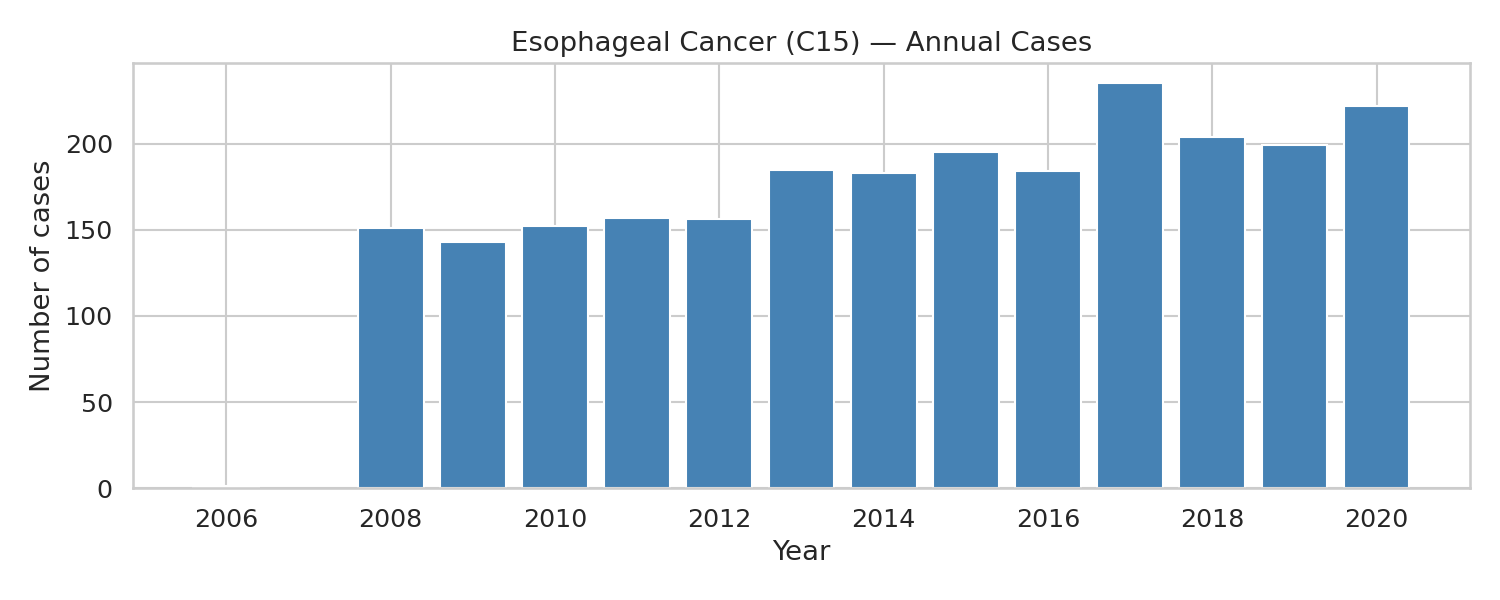
\includegraphics[width=0.95\linewidth]{02_descriptive/fig_incidence_trend.png}
  \caption{\textbf{Annual incidence trend.}
    Annual case volume of esophageal cancer (ICD-10 C15) at the study
    centre (2006--2020). A modest increasing trend is observed, consistent
    with an ageing population and improving endoscopic detection of
    early-stage lesions.}
  \label{fig:chars}
\end{figure}

\clearpage

\begin{figure}[H]
  \centering
  \begin{subfigure}[t]{0.48\linewidth}
    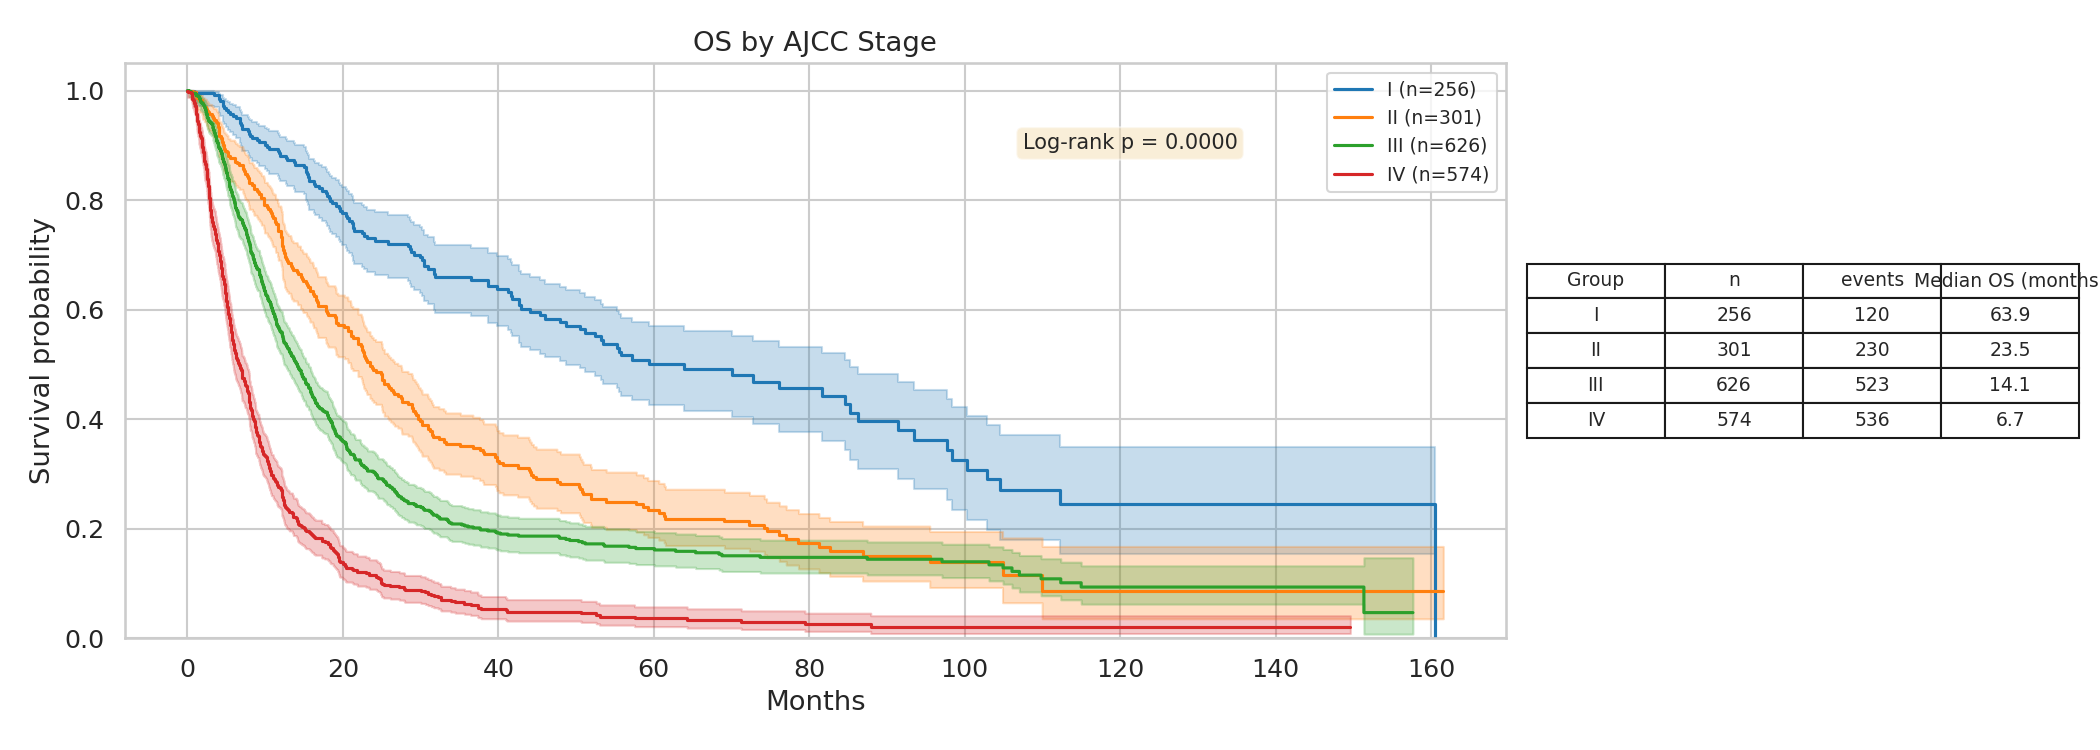
\includegraphics[width=\linewidth]{03_survival/km_stage.png}
    \caption{OS by AJCC stage}
  \end{subfigure}
  \hfill
  \begin{subfigure}[t]{0.48\linewidth}
    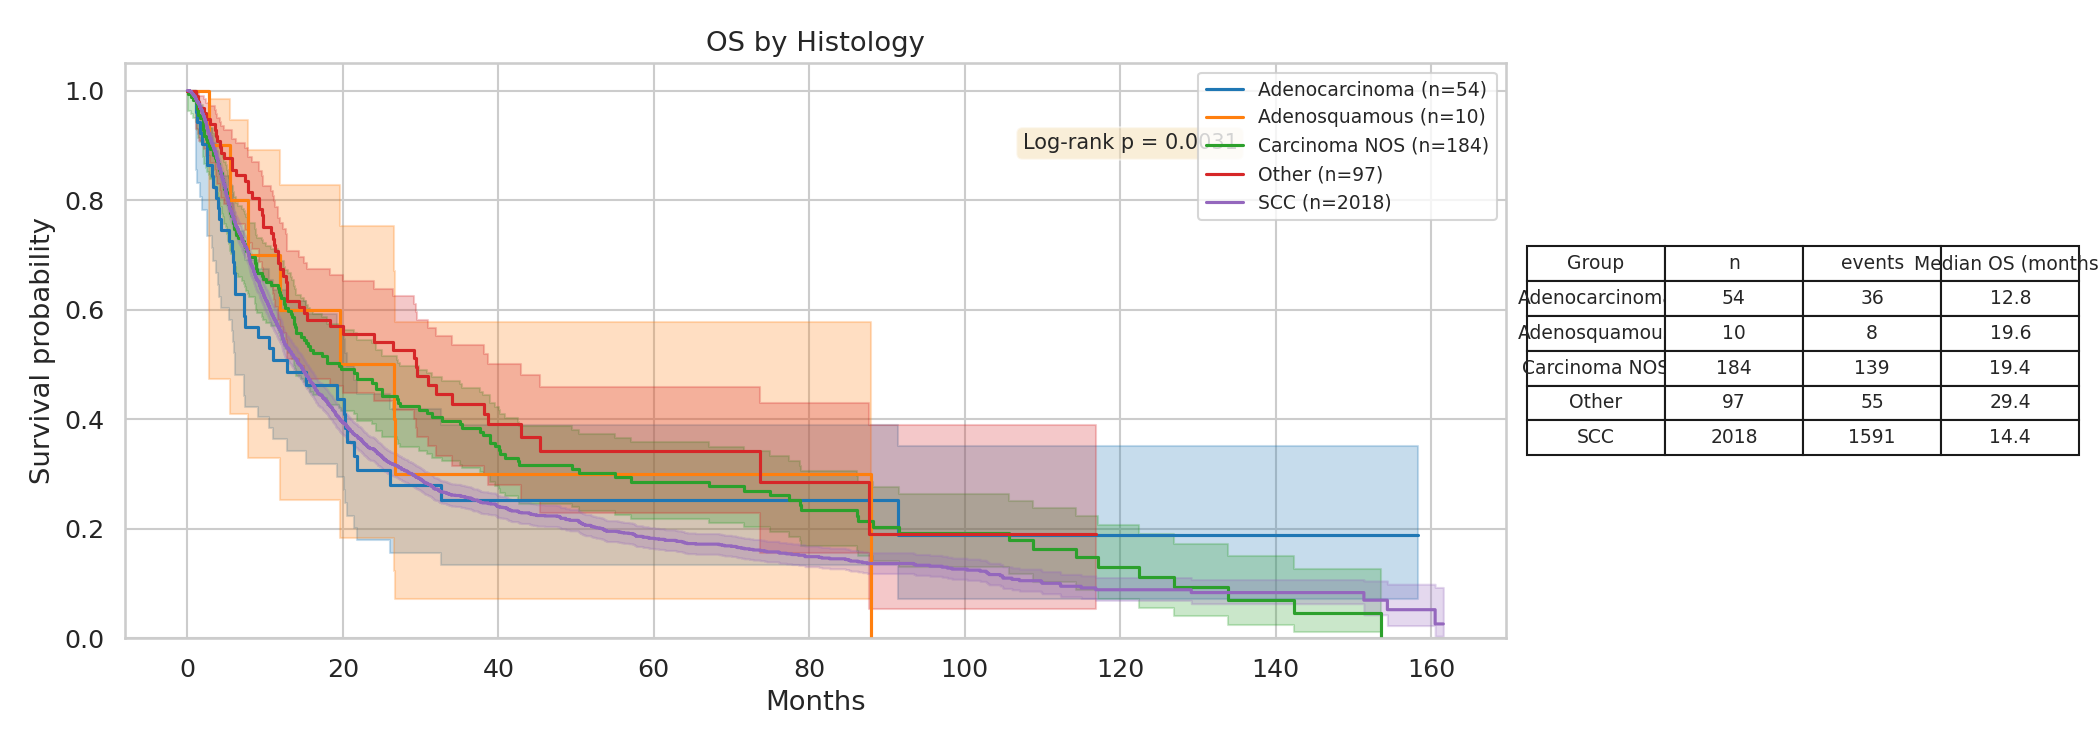
\includegraphics[width=\linewidth]{03_survival/km_histology.png}
    \caption{OS by histological type}
  \end{subfigure}
  \caption{\textbf{Overall survival by stage and histology.}
    Kaplan-Meier curves of overall survival stratified by (A) AJCC
    pathological/clinical stage and (B) histological type. Shaded areas
    represent 95\,\% confidence intervals; $p$-values are from the
    log-rank test. Note: adenocarcinoma subgroup ($n = 54$) is
    hypothesis-generating only; the small sample size precludes
    reliable independent survival estimation.}
  \label{fig:km_stage_hist}
\end{figure}

\clearpage

\begin{figure}[H]
  \centering
  \begin{subfigure}[t]{0.48\linewidth}
    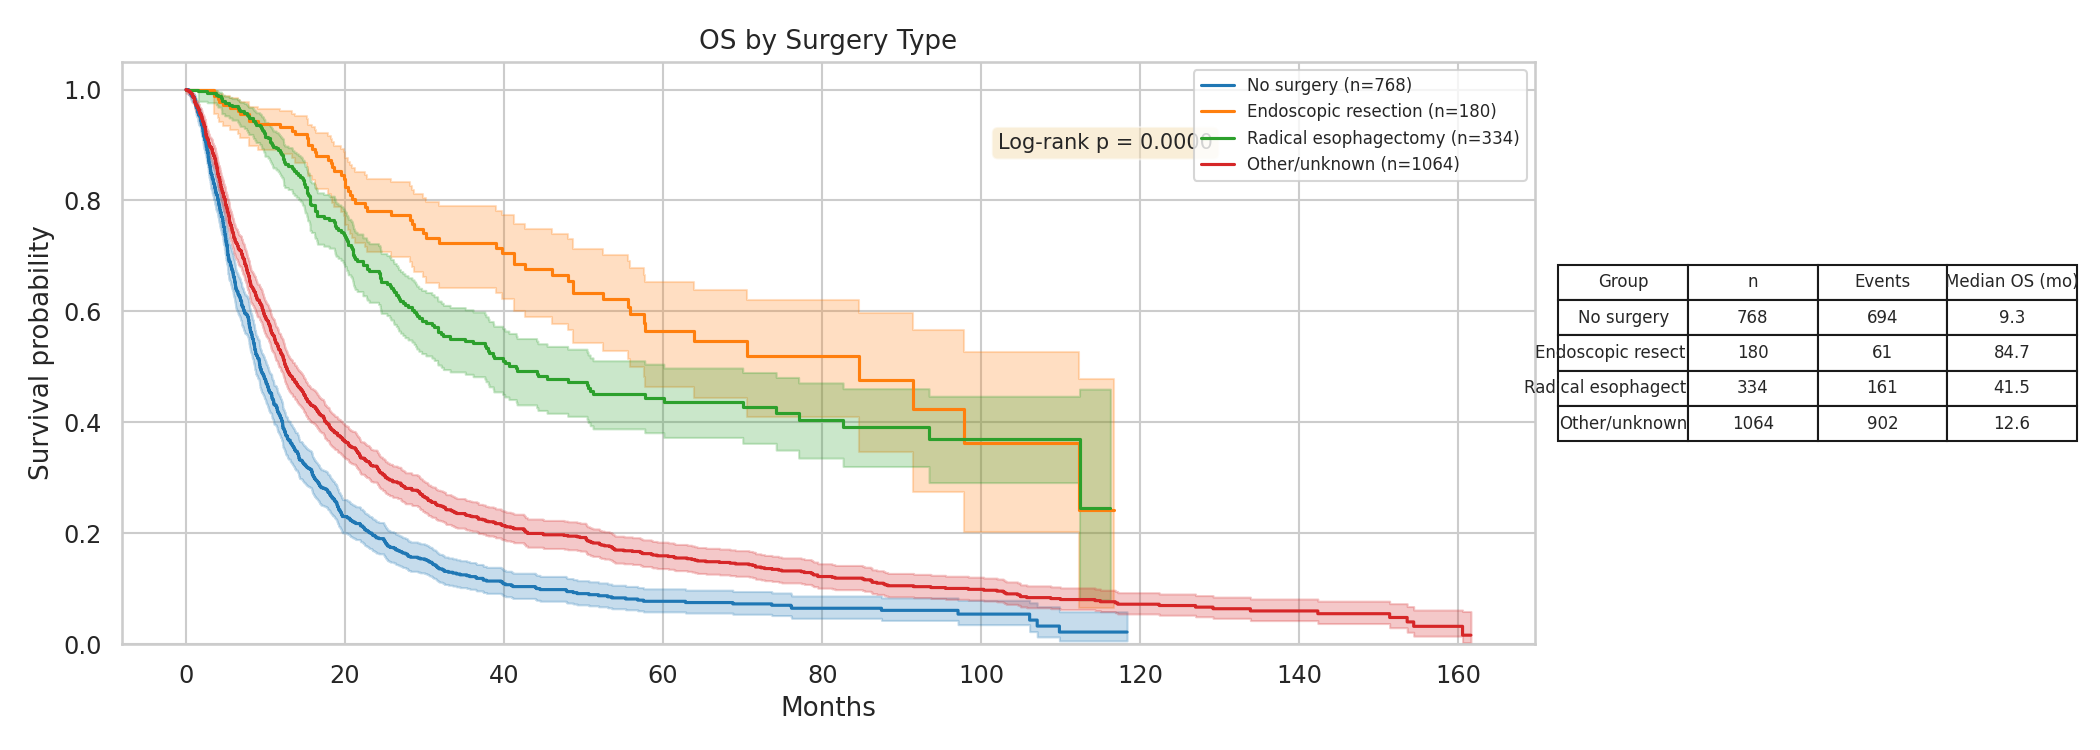
\includegraphics[width=\linewidth]{06_chemo_surgery/km_surgery_type.png}
    \caption{OS by surgical modality}
  \end{subfigure}
  \hfill
  \begin{subfigure}[t]{0.48\linewidth}
    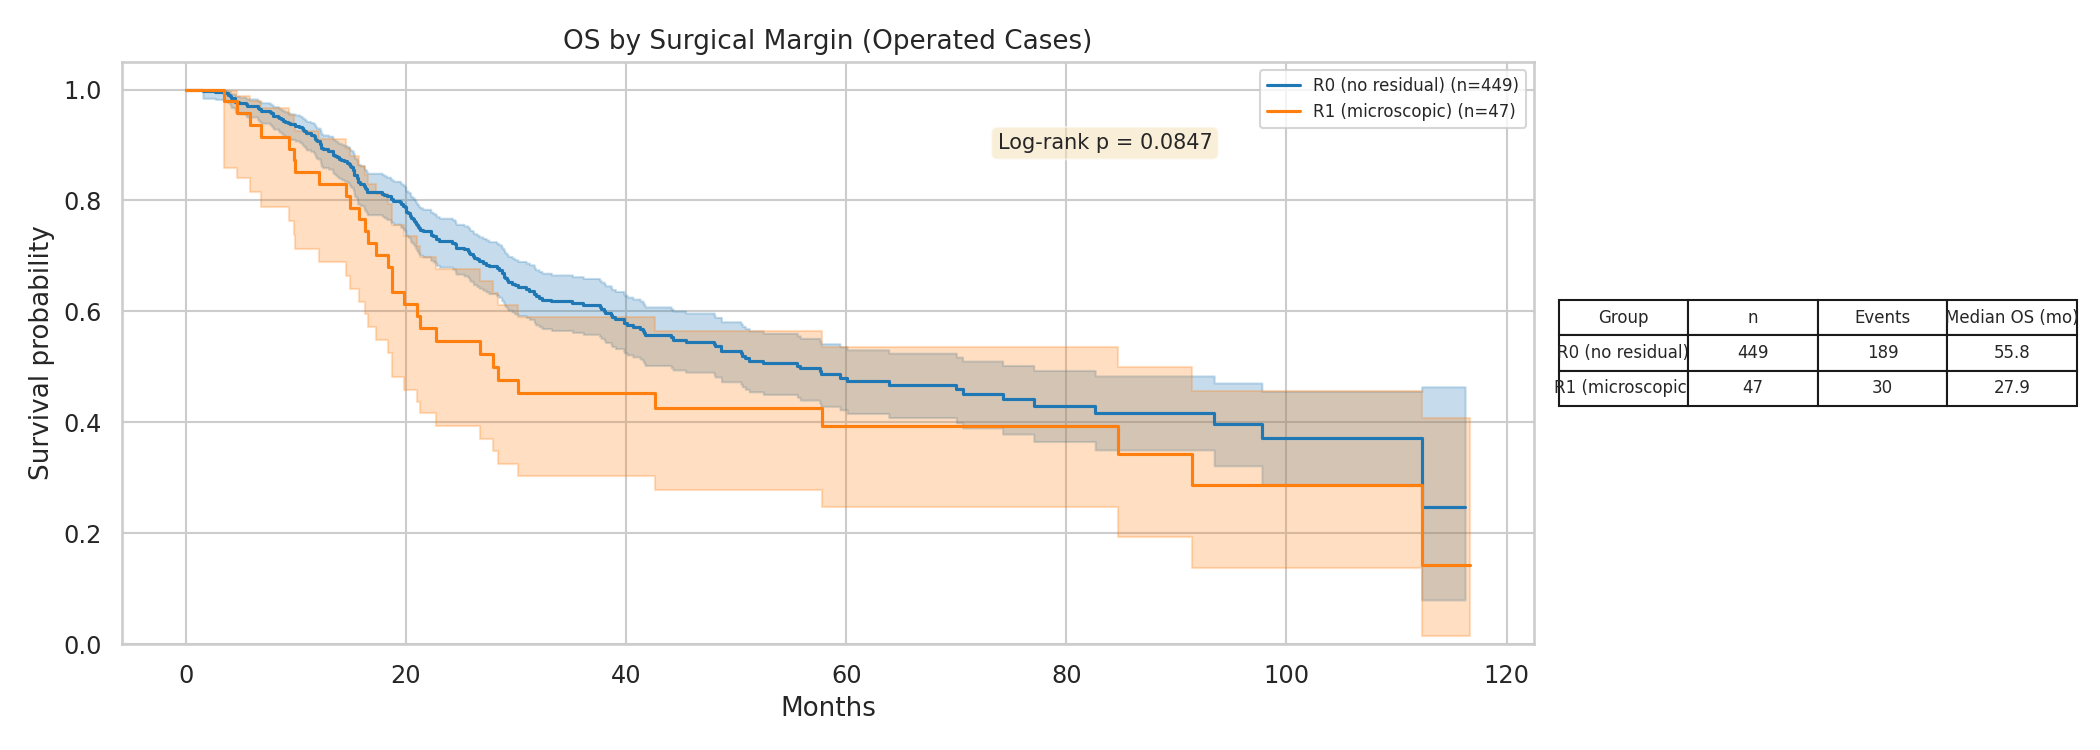
\includegraphics[width=\linewidth]{06_chemo_surgery/km_surgery_margin.png}
    \caption{OS by resection margin (operated)}
  \end{subfigure}
  \caption{\textbf{Surgical outcomes.}
    (A) Overall survival stratified by surgical modality; no surgery is
    the reference. (B) OS by resection margin status (R0 vs R1) among
    operated patients. The superiority of endoscopic resection reflects
    selection toward early-stage disease.}
  \label{fig:surgery}
\end{figure}

\clearpage

\begin{figure}[H]
  \centering
  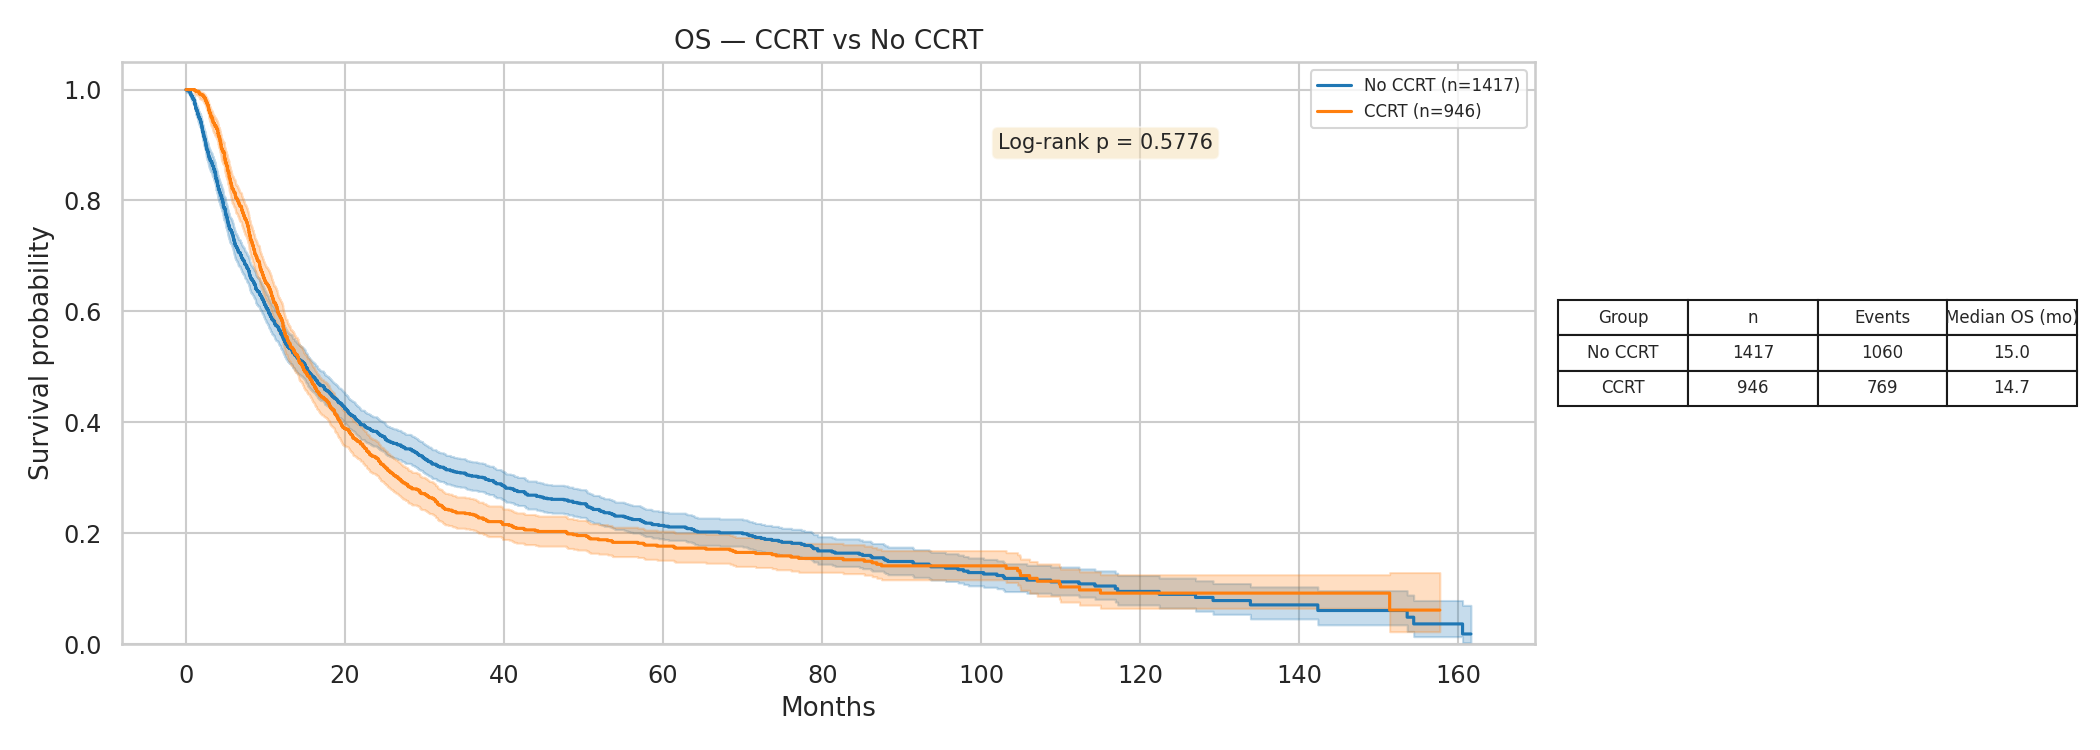
\includegraphics[width=0.65\linewidth]{06_chemo_surgery/km_ccrt.png}
  \caption{\textbf{Overall survival by CCRT status (unadjusted Kaplan-Meier).}
    Unadjusted Kaplan-Meier curves for CCRT vs non-CCRT patients
    (log-rank $p = 0.58$, non-significant). Three adjusted estimates are
    reported: MICE primary HR 0.97 ($p = 0.569$, consistent with
    unadjusted result); complete-case staged patients HR 0.72
    ($p < 0.001$); zero-coded stage HR 0.76 ($p < 0.001$, likely
    artefactual). The $>$25\,\% MICE vs complete-case divergence
    precludes a definitive conclusion (see §3.5 and §4.2).}
  \label{fig:chemo}
\end{figure}

\clearpage

\begin{figure}[H]
  \centering
  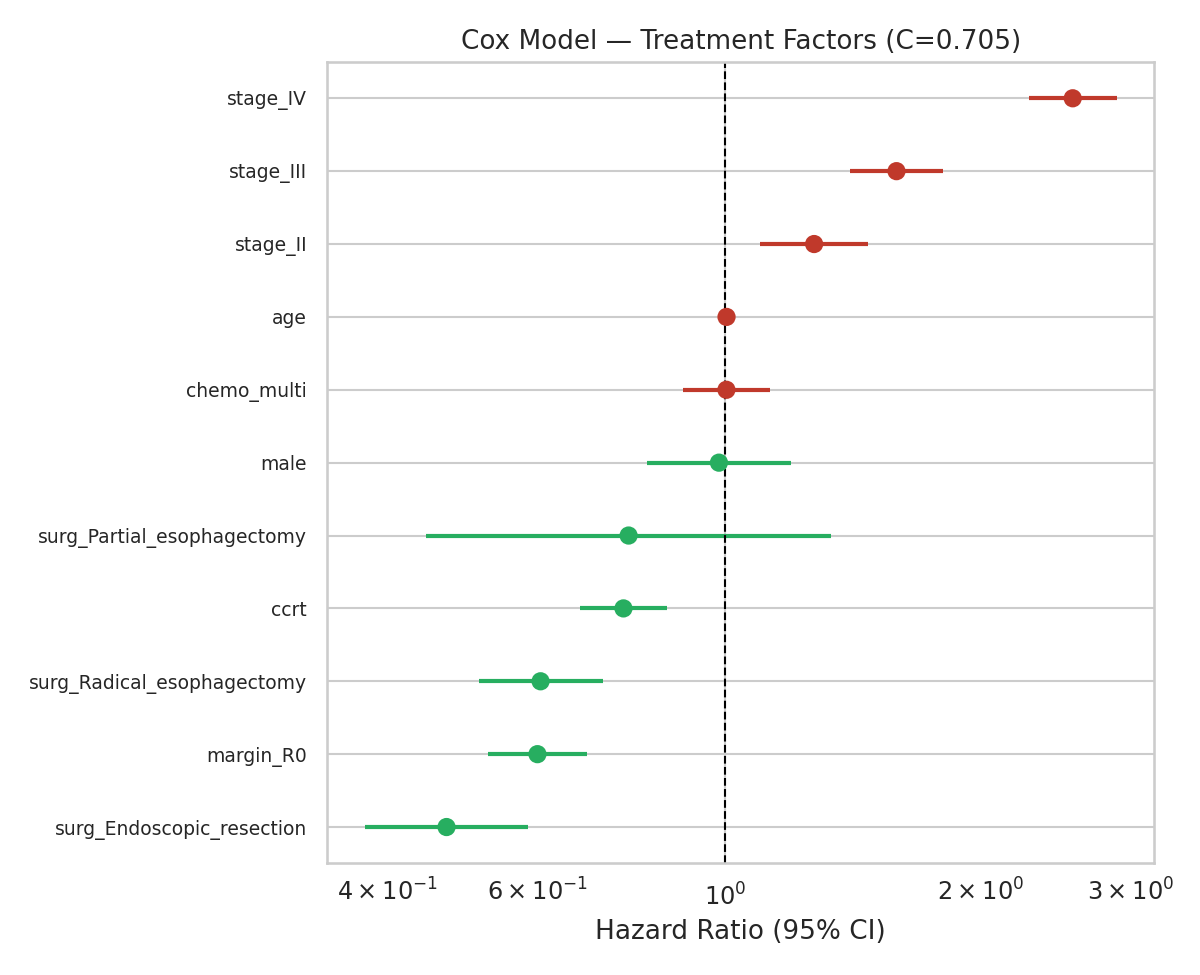
\includegraphics[width=0.92\linewidth]{06_chemo_surgery/cox_treatment_forest.png}
  \caption{\textbf{Multivariable Cox proportional hazards forest plot ---
    treatment predictors.}
    Hazard ratios (HR) with 95\,\% confidence intervals for surgical and
    systemic treatment predictors in the full adjusted model
    ($n = 2{,}364$; primary MICE-imputed stage analysis, C-index 0.670).
    Covariates adjusted for age, sex, and MICE-imputed AJCC stage.
    Note: three CCRT estimates --- MICE primary HR 0.97 ($p = 0.569$,
    NS); complete-case staged patients HR 0.72 ($p < 0.001$);
    zero-coded stage HR 0.76 ($p < 0.001$, likely artefactual) ---
    see Table~\ref{tab:cox} footnote and Results §3.5.
    Reference: no surgery, R1/R2 margin, no CCRT.
    ***$p < 0.001$, **$p < 0.01$, *$p < 0.05$, ns: not significant.}
  \label{fig:cox}
\end{figure}

\clearpage

\begin{figure}[H]
  \centering
  \begin{subfigure}[t]{0.48\linewidth}
    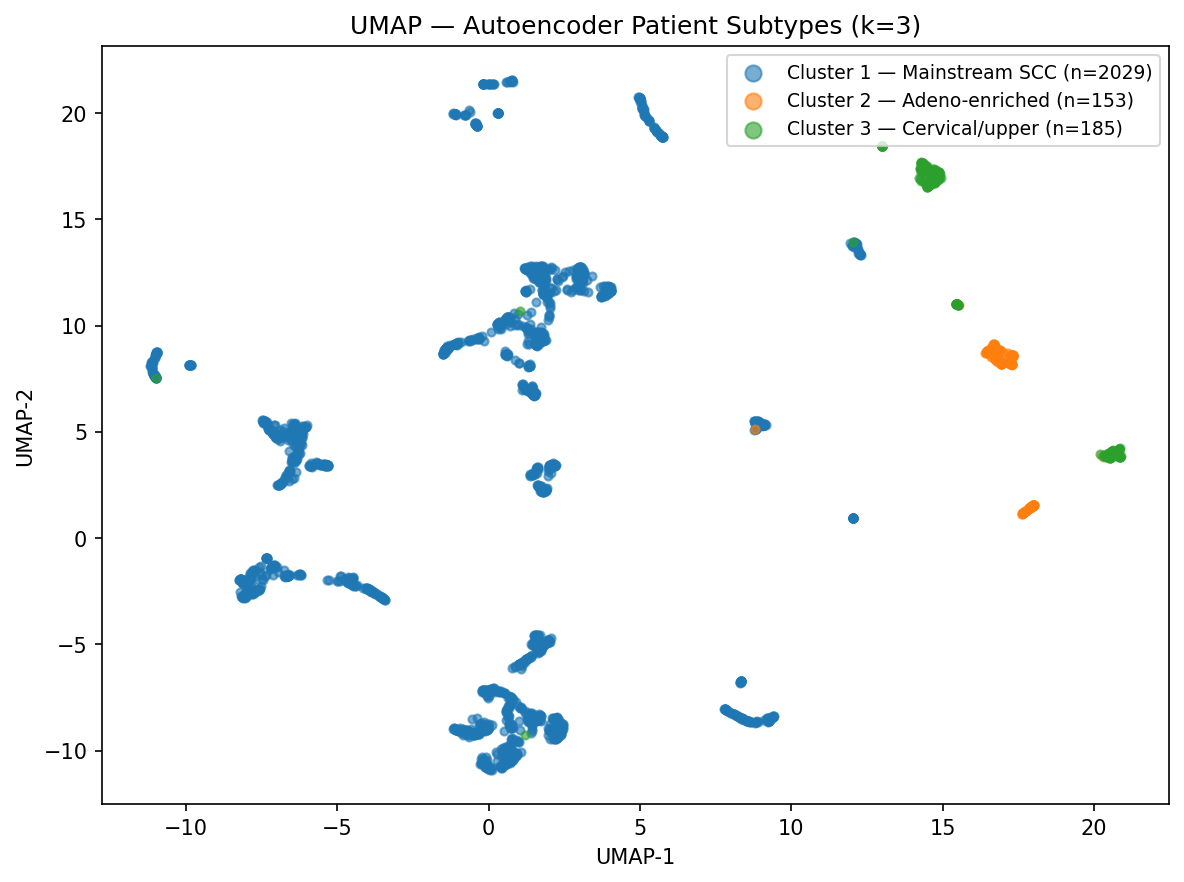
\includegraphics[width=\linewidth]{04_deep_learning/umap_kmeans_k3.png}
    \caption{UMAP coloured by cluster}
  \end{subfigure}
  \hfill
  \begin{subfigure}[t]{0.48\linewidth}
    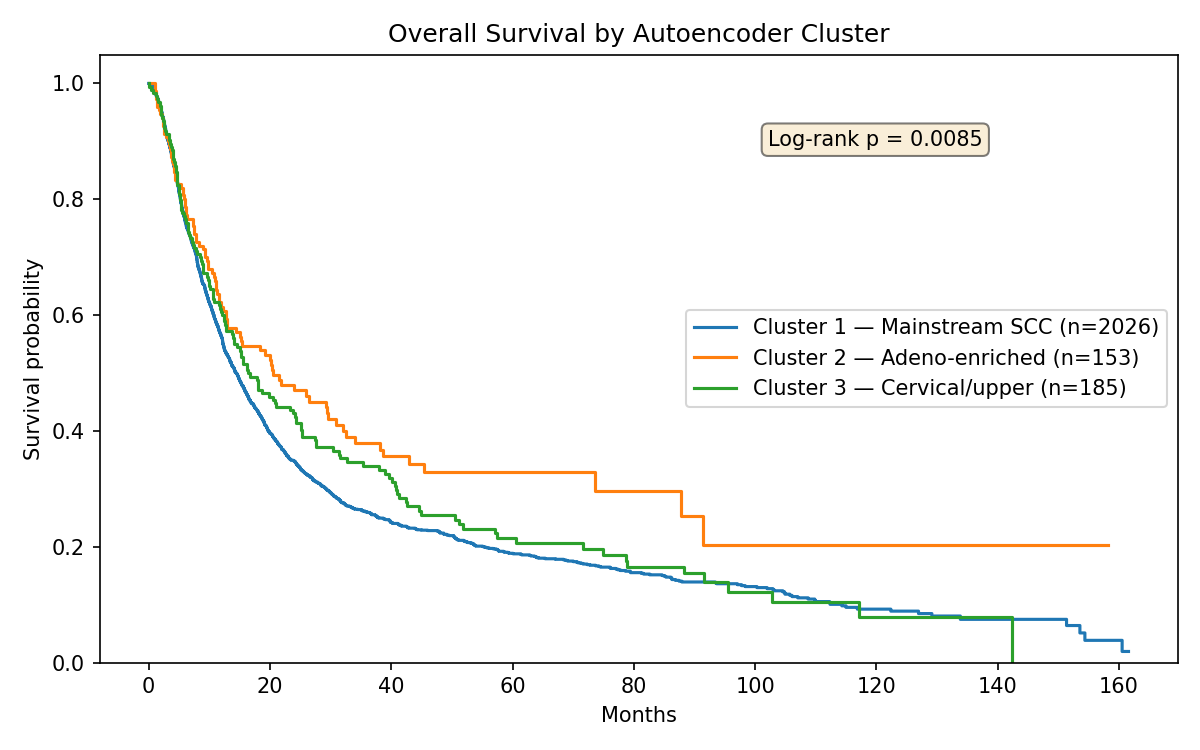
\includegraphics[width=\linewidth]{04_deep_learning/km_clusters_k3.png}
    \caption{OS by autoencoder cluster}
  \end{subfigure}
  \caption{\textbf{Deep learning patient subtype discovery.}
    (A) UMAP two-dimensional embedding of the autoencoder 8-dimensional
    latent space, coloured by $k$-means cluster assignment ($k = 3$).
    Substantial overlap between clusters in the UMAP projection is
    consistent with the partial separation of subtypes within the
    latent space; OS differences across clusters reflect in part
    composition by known prognostic subgroups (histology and subsite).
    (B) Kaplan-Meier overall survival curves by cluster (log-rank
    $p = 0.009$). Cluster~1 = mainstream SCC ($n = 2{,}026$);
    Cluster~2 = adenocarcinoma-enriched ($n = 153$);
    Cluster~3 = cervical/upper-esophagus ($n = 185$).
    KM analysis: 3 patients excluded due to missing follow-up (total
    cluster assignments $n = 2{,}367$).}
  \label{fig:dl}
\end{figure}

\clearpage

\begin{figure}[H]
  \centering
  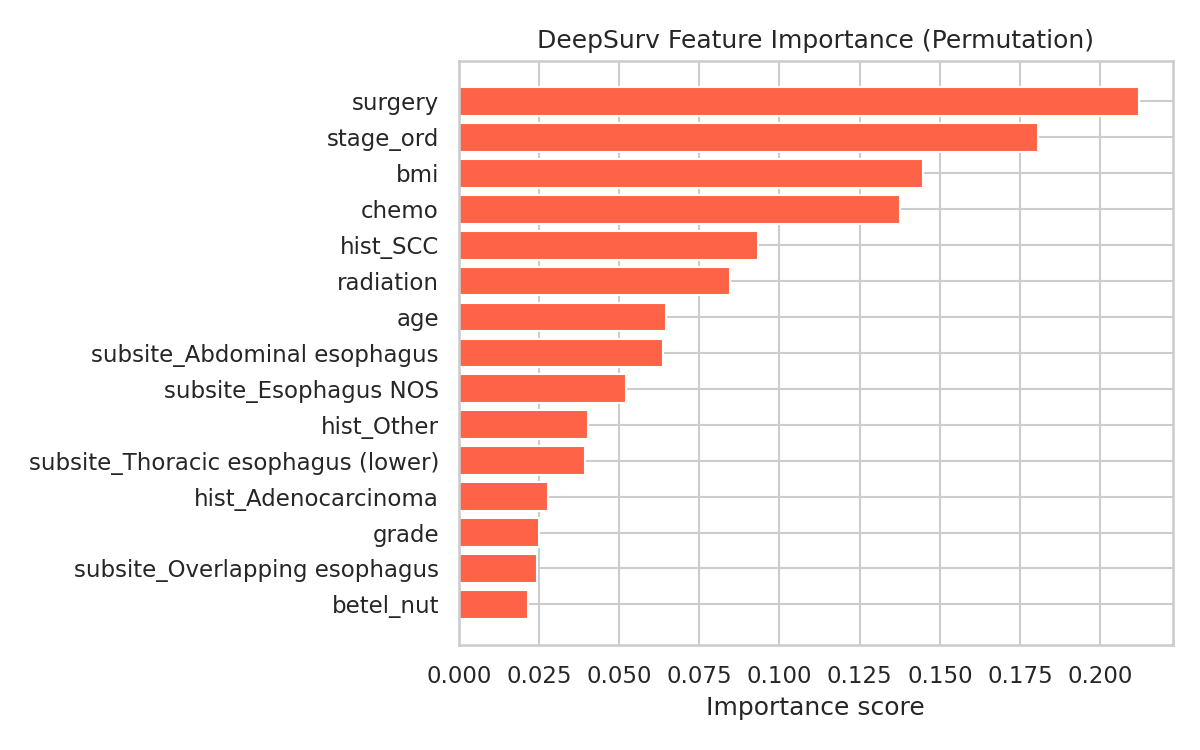
\includegraphics[width=0.75\linewidth]{04_deep_learning/deepsurv_feature_importance.png}
  \caption{\textbf{DeepSurv permutation feature importance.}
    Feature importance estimated by permuting each clinical variable
    and quantifying the resulting change in concordance. Variable labels
    reflect internal coding: \texttt{surgery} = any surgical resection;
    \texttt{stage\_ord} = AJCC stage (ordinal 1--4); \texttt{chemo} =
    any chemotherapy; \texttt{hist\_SCC} = SCC histology.
    Surgery, AJCC stage, and chemotherapy are the three strongest
    discriminators of risk, consistent with the multivariable Cox model
    (Table~\ref{tab:cox}).}
  \label{fig:deepsurv}
\end{figure}

\end{document}
